\section{Мета}
Вивчення організації буфера клавіатури та набуття практичних навичок визначення збережених у буфері ASCII та скан-кодів клавіш клавіатури.


\section{Завдання}
Визначте ASCII код англійської літери, номер якої в алфавіті збігається з номером студента в журналі.
Визначити скан-код цієї клавіши.


\section{Хід роботи}
\subsection{Код програми}
\lstinputlisting[language=Rust, style=colouredRust]{\codeDirectory/lab5/main.c}

\subsection{Результат роботи програми}
\begin{figure}[ht!]
    \centering
    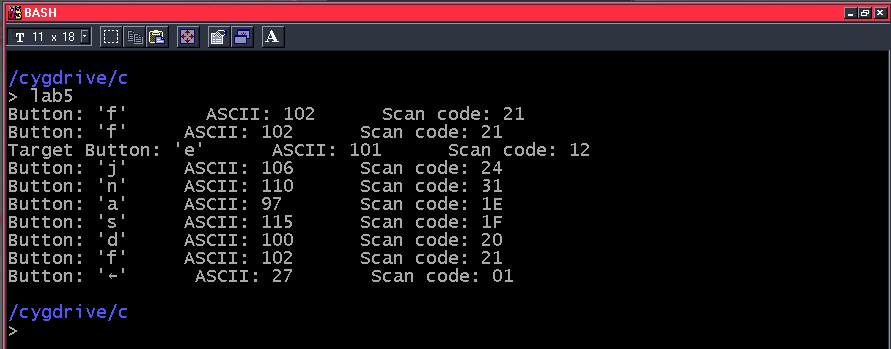
\includegraphics[width=0.9\textwidth]{\assetsDirectory/lab5.png}
    \caption{Результат роботи програми}
\end{figure}

\clearpage
\section{Висновки}
У процесі виконання практичної роботи було досліджено структуру організації буфера клавіатури. Отримано практичні навички зчитування та аналізу ASCII-кодів і скан-кодів клавіш, збережених у буфері клавіатури.
